\documentclass{article}
\usepackage[utf8]{inputenc} 			%deutsche Umlaute
\usepackage[ngerman]{babel} 			%deusche Sprache
\usepackage{graphicx}

\title{Fachprojekt Digital Entertainment Technologies Wintersemester 19/20}
\author{KÄSEBROT\\
Julia Linnenberg  \\
		Lisa Roth\\	
	Technische Universität Dortmund \\
	}
\date{\today}
\begin{document}
\maketitle
\section{Zwischenstand 14. Januar 2020}
\begin{itemize}

\item Löcher Problem wurde gefixt

\item "Hier nicht Graben" - Schild wird zufällig gesport, darunter befindet sich der Blocktype "HELGE"
\item Wenn man den Blocktype Helge zerstört, werden dort Mumien gespawnt
\item Mumien fliegen auf den Player zu und schreien dabei

\item Welt wird zu Beginn im Radius von 8 Chunks gebaut
\item Chunks zerstören sich nicht mehr

\item (zufällige) Level ID setzt Level: \{0..359\}
$\rightarrow$ Wasserseed: LevelID modulo 10 + 1 $\Rightarrow$ 10 verschiedene Wasserhäufigkeiten\\
$\rightarrow$ Kaktusseed: float cs = (levelID modulo 60)/10 $\Rightarrow$ 6 verschiedene Kaktushäufigkeiten\\
$\rightarrow$ Positionseed: LevelID/60  $\Rightarrow$ 6 verschiedene Landschaften\\

\end{itemize}
\begin{center}
\begin{figure}
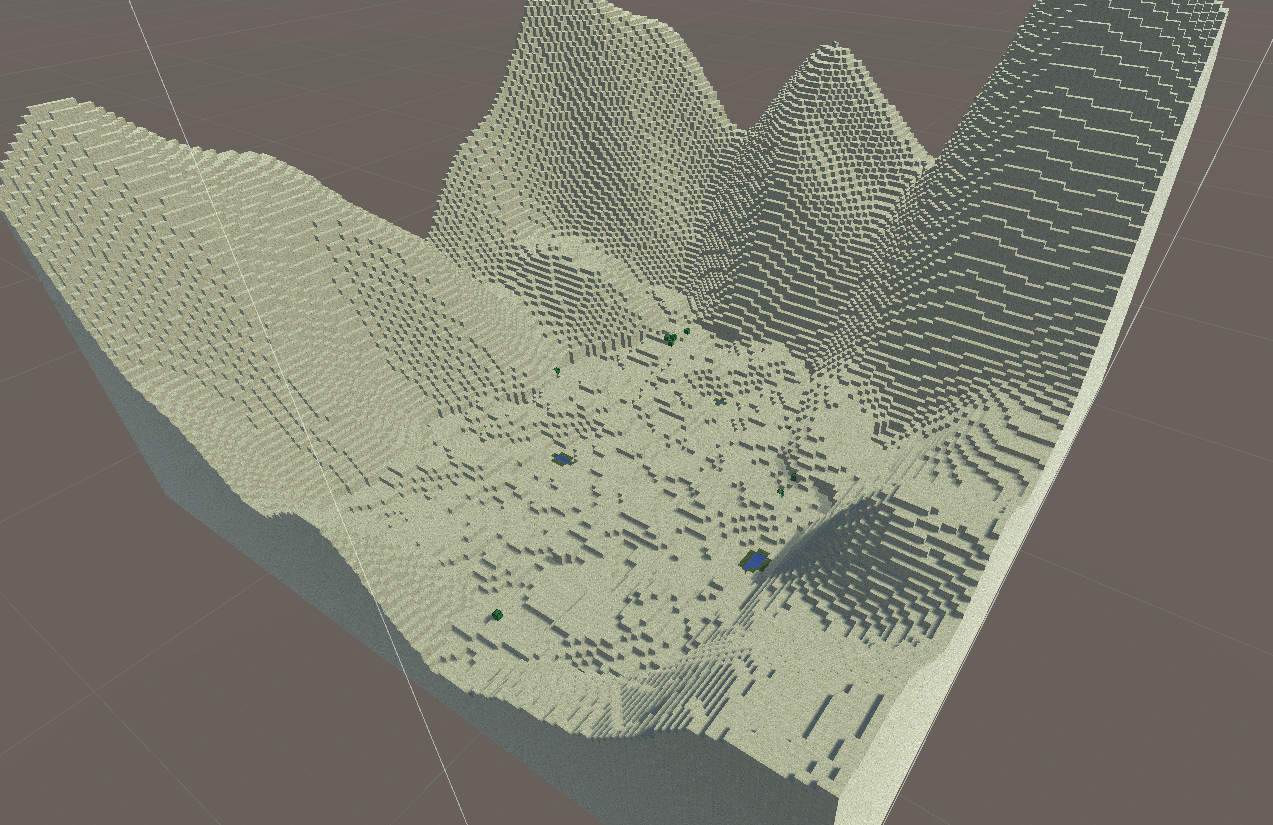
\includegraphics[width=\textwidth]{level0_1.png}
\caption{Level 0 $\rightarrow$ wenige Kakteen, wenig Wasser}
\end{figure}
\begin{figure}
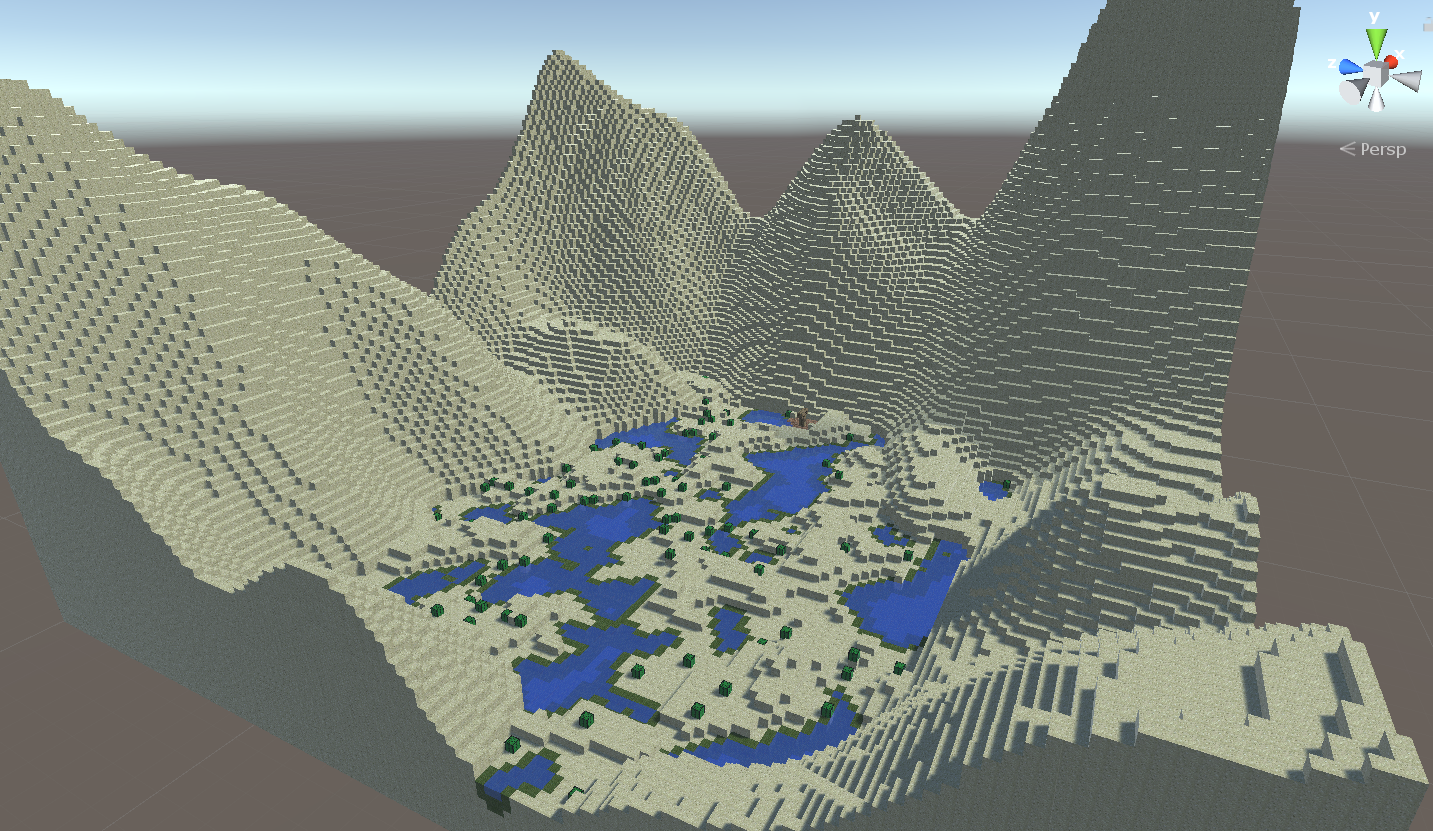
\includegraphics[width=\textwidth]{level59_1.png}
\caption{Level 0 $\rightarrow$ viele Kakteen, viel Wasser}
\end{figure}
\begin{figure}
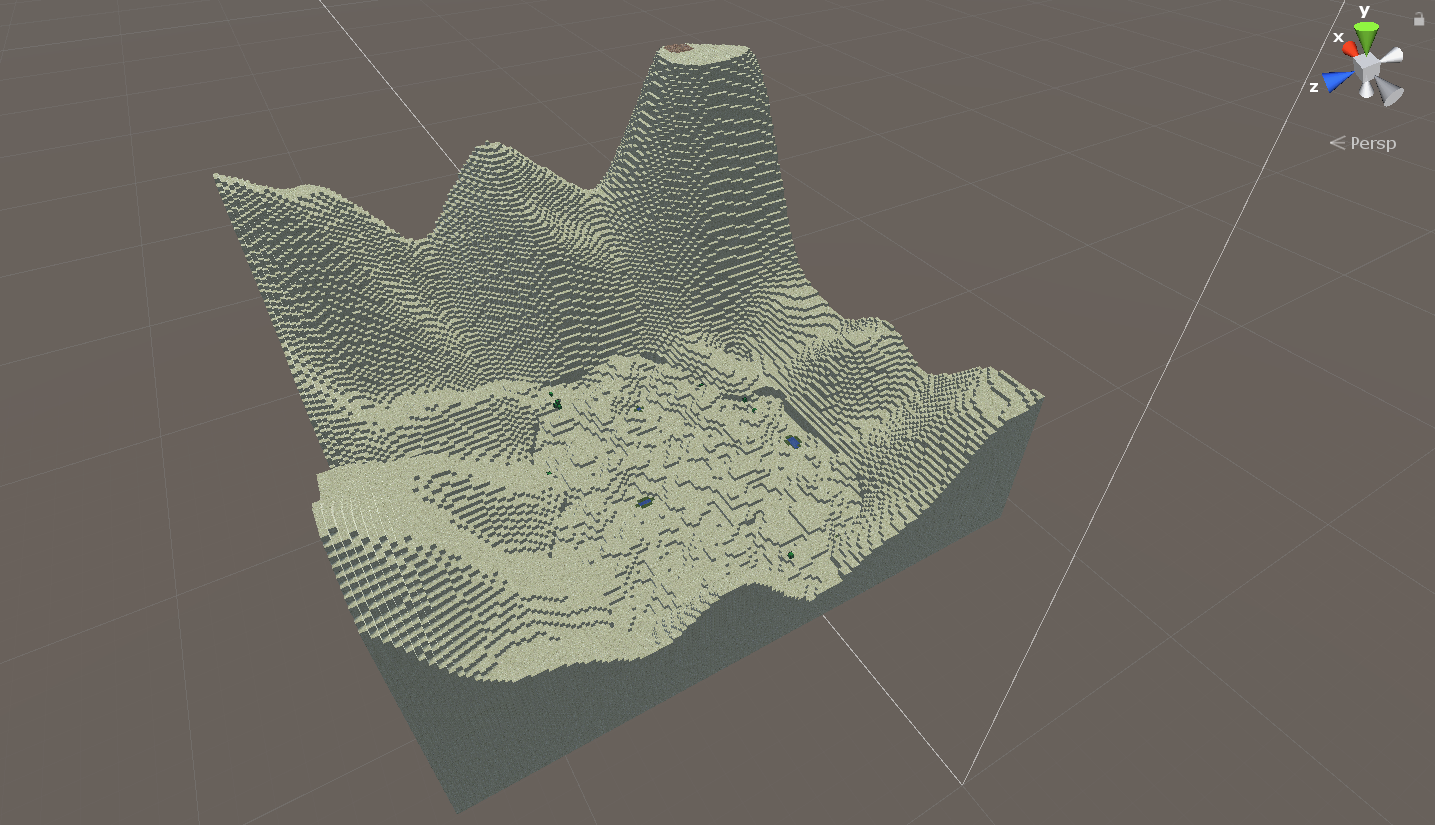
\includegraphics[width=\textwidth]{level0.png}
\caption{Level 0 $\rightarrow$ wenig Kakteen, wenig Wasser}
\end{figure}
\end{center}
\end{document}